\documentclass[12pt, A4]{report}

% Packages
	% Basics
		\usepackage{amsmath}
		\usepackage{bm}
		\usepackage{cellspace}
		\usepackage{cite}
		\usepackage{csquotes}
		\usepackage{fixltx2e}
		\usepackage[hang,flushmargin]{footmisc}
		\usepackage{float}
		\usepackage[margin=0.75in]{geometry}
		\usepackage{graphicx}
		\usepackage{hyperref}
		\usepackage[utf8]{inputenc}
		\usepackage{subcaption}
	% Diagrams
		\usepackage{pgfplots}
		\usepackage{tikz}
			\usepackage{circuitikz} % Circuits
			\usepackage{tikz-3dplot} % 3D
			\usetikzlibrary{arrows.meta, angles, calc, quotes}
	% Notation
		\usepackage{amssymb} % Miscellaneous
		\usepackage{chemformula}
		\usepackage{esint} % Integrals
		\usepackage{physics} % Differentials/Vectors
% Macros
	% Notation
		% Constants
			\DeclareMathOperator{\en}{e}
		% Distributions
			\newcommand{\Exp}{\mathbb{E}}
			\newcommand{\ndist}{\mathcal{N}}
			\DeclareMathOperator{\vari}{var}
		% Functions
			\DeclareMathOperator{\erfc}{erfc}
		% Sets
			\newcommand{\R}{\mathbb{R}}
		% Other
			\DeclareMathOperator{\avg}{avg}
			\renewcommand{\th}{\text{th}}
	% Utilities
		\newcommand{\callout}[2]{\begin{center}\fbox{\begin{minipage}{#1cm}#2\end{minipage}}\end{center}}
		\newcommand{\comment}[1]{}
		\newcommand{\subsectionb}[1]{\subsection*{#1}\addcontentsline{toc}{subsection}{#1}}
		\newcommand{\subsubsectionb}[1]{\subsubsection*{#1}\addcontentsline{toc}{subsubsection}{#1}}

% Configuration
	\title{Differential Equations Project: Phase 3}
	\author{Arnav Patri and Shashank Chidige}
	\date{}
	\hypersetup{
	    colorlinks,
	    citecolor=cyan,
	    filecolor=cyan,
	    linkcolor=cyan,
	    urlcolor=cyan
	}
	\cellspacetoplimit10pt
	\cellspacebottomlimit10pt


\begin{document}
	\maketitle
	\noindent
	Table 1 shows information regarding Alphabet Inc., which is listed on the New York Stock Exchange as GOOG, as the company used to be known as Google. The data is taken from Yahoo Finance \cite{Yahoo}, which provides financial news and data for public use. The domain of the independent variable, time (\(t\)) is taken from 9/27/2022 to 10/15/2022.
	\[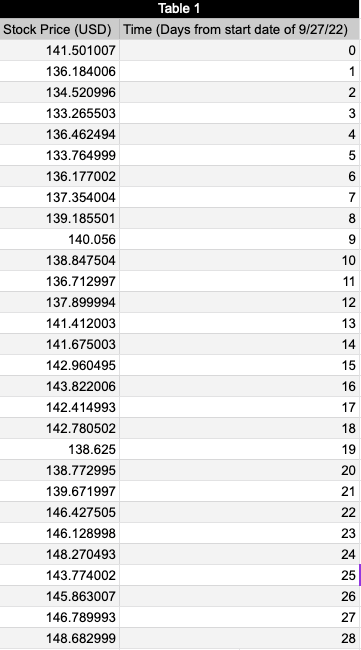
\includegraphics[width = 9cm]{Images/Table_1}\]
	Table 2 shows the differential approach to deriving the differential equation model. As the stochastic part cannot be derived, only the derivation of the deterministic part is shown. Columns 1 and 2 are simply copied from Table 1. Equations 1 and 2 are used to derive the changes in stock price \(S_t\) and time \(t\), put into columns 3 and 4 respectively. The derivative of \(S_t\) with respect to \(t\) can be approximated as \(\Delta S_t/\Delta t\), as shown in column 5. The stock price \(S_t\) is then listed again, as the plot is of \(\Delta S_t/\Delta t\) vs \(S_t\).
	\[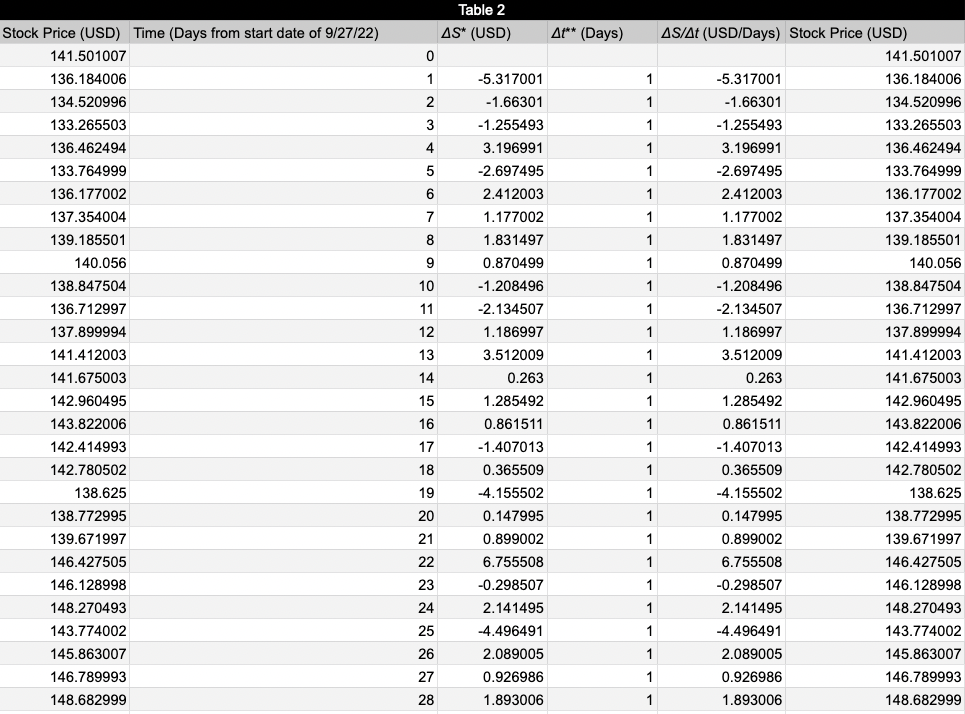
\includegraphics[width = 18cm]{Images/Table_2}\]
	\begin{align*}
		\Delta S_i &= S_i - S_{i - 1} \tag{Equation 1*} \\
		\Delta t_i &= t_{i} - t_{i - 1} \tag{Equation 2**}
	\end{align*}
	This is the graph of \(\Delta S/\Delta t\) (in USD/day) vs \(S\) (in USD) with a linear regression performed.
	\[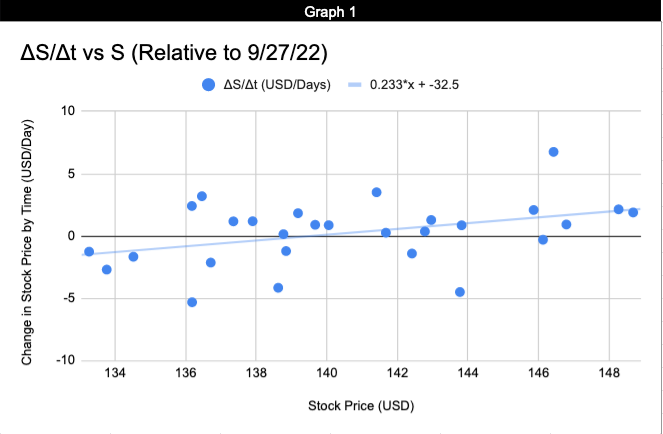
\includegraphics[width = 10cm]{Images/Graph_1}\]
	It is clear that there is a linear relationships between the stock price and its derivative with respect to time. It can therefore be said that
		\[
			\dv{S_t}{t} \propto S_t \implies \dv{S}{t} = \mu S_t
		\]
		where \(\mu\) is a constant. Using information from Stochastic Calculus: An Introduction with Applications \cite{Stochastic}, the Wiener process, which was previously discussed in Phase 2, can be appended, adding the random motion to the model:
		\[
			\dv{S_t}{t} = \mu S_t + \sigma S_t\dv{W_t}{t}
		\]
		where \(S_t\) is stock price as a function of time \(t\), \(\mu\) is the (constant) drift, \(\sigma\) is the (constant) volatility, and \(W_t\) is a standard Wiener process. The dependent variable \(t\) is not present, making this an autonomous DE. The only information needed for the model are \(\mu\), \(\sigma\), and the initial stock price \(S_0\). \\
	\(\mu\) is the amount that \(\Exp(S_t)\), the expected value of the stock price, changes per year, making it the coefficient of the linear regression of \(\Delta S/\Delta t\) against \(S\) divided by 365, so \(\mu \approx 0.00064\).\\
	\(\sigma\) is simply the standard deviation of the stock price in the sample, so 
		\[\sigma = \sqrt{\frac{\sum\limits_{i = 1}^n(S_{t, i} - \bar{S}_{t})^2}{n - 1}} \approx 4.356\]
		where \(n\) is the number of days sampled, \(S_{t, 1 \cdots n}\) are the particular stock prices, and \(\bar{S}_t\) is the average stock price in the sample:
		\[\bar{S}_t = \frac{\sum\limits_{i = 1}^nS_{t,i}}{n}\]
	The model then becomes
		\[\boxed{\dv{S_t}{t} = 0.00064S_t + 4.356S_t\dv{W_t}{t}}\]
	\begin{thebibliography}{1}
		\bibitem{Yahoo}
			Yahoo Finance,
			\textit{Alphabet Inc. (GOOG) Stock Price, News, Quote \& history - Yahoo Finance},
			New York, NY,
			2022.
		\bibitem{Stochastic}
			Gregory F. Lawler,
			\textit{Stochastic Calculus: An Introduction with Applications},
			Chicago, IL, 
			2014.
	\end{thebibliography}
\end{document}
